% This is a basic Math Paper

\documentclass[11pt]{article}

% Preamble

\usepackage[margin=1in]{geometry}
\usepackage{amsfonts, amsmath, amssymb}
\usepackage{fancyhdr, float, graphicx}
\usepackage[utf8]{inputenc} % Required for inputting international characters
\usepackage[T1]{fontenc} % Output font encoding for international characters
\usepackage{fouriernc} % Use the New Century Schoolbook font
\usepackage[nottoc, notlot, notlof]{tocbibind}
\usepackage{url}

% Header and Footer
\pagestyle{fancy}
\fancyhead{}
\fancyfoot{}
\fancyhead[L]{\textit{\Large{Working of Turbines}}}
%\fancyhead[R]{\textit{something}}
\fancyfoot[C]{\thepage}
\renewcommand{\footrulewidth}{1pt}



% Other Doc Editing
% \parindent 0ex
%\renewcommand{\baselinestretch}{1.5}

\begin{document}
	
	\begin{titlepage} 
		\centering 
		
		%---------------------------NAMES-------------------------------
		
		\huge\textsc{
			MIT World Peace University
		}\\
	
		\vspace{0.75\baselineskip} % space after Uni Name
		
		\LARGE{
			Digital Thinking Laboratory\\
			First Year B. Tech, Trimester 2
		}
		
		\vfill % space after Sub Name
		
		%--------------------------TITLE-------------------------------
		
		\rule{\textwidth}{1.6pt}\vspace*{-\baselineskip}\vspace*{2pt}
		\rule{\textwidth}{0.6pt}
		\vspace{0.75\baselineskip} % Whitespace above the title
		
		
		
		\huge{\textsc{
				Design Idea for Dimly Lit Roads in India\\
				"Grabus"
			}} \\
		
		
		
		\vspace{0.5\baselineskip} % Whitespace below the title
		\rule{\textwidth}{0.6pt}\vspace*{-\baselineskip}\vspace*{2.8pt}
		\rule{\textwidth}{1.6pt}
		
		\vspace{1\baselineskip} % Whitespace after the title block

		%--------------------------SUBTITLE --------------------------	
			
		\LARGE\textsc{
			Project Report for a Design Idea in the\\ \underline{Public Utility and Civil Sector}
		} % Subtitle or further description
		\vfill
		
		%--------------------------AUTHOR-------------------------------
		
		Prepared By
		\vspace{0.5\baselineskip} % Whitespace before the editors
		
		\Large{
			54. Krishnaraj Thadesar\\ 45. Pranaav Suratwala\\
			44. Devanshu Surana\\56. Tirth Thesiya\\
			Division 9 Batch I3
		}
		
		
		\vspace{0.5\baselineskip} % Whitespace below the editor list
		\today

	\end{titlepage}
	
	
\tableofcontents
\thispagestyle{empty}
\clearpage


\setcounter{page}{1}

\section{Introduction}
In this Project, we will try to solve the Problem of Dimly Lit Roads in India and any other Part of the world, with the Intention of Generating Renewable Clean Electrical Energy that can be supplied to street Lights. We will Look over some of the alternate Solutions that were brought up as part of the General discussion as part of this Activity. We will see why Some of those ideas worked and others did not. \\

We will then look at the Proposed Design, the Materials Used in said design, and its prototypes, Sketches and Diagrams. It's Estimated Energy Generation will be discussed along with the Best case and Worst Case Scenario, which will correspond to weather or not there is a Profit Margin. \\

Its Potential Merits, Demerits and Learning Experiences will be discussed as well along with the Environmental Impacts, 

\section{Problem Statement}

\begin{quote}
	\textit{"Many Roads in India and Other Parts of the World are Dimly Lit because of Absense of Electricity for Street Lights"}
\end{quote}
While City Corporations claim that more than 90 Percent of the conventional street lights in the city have been converted into LED lights to provide better illumination, several roads in the city still remain pitch dark. Even the arterial roads including VOC Road near the Central bus stand lack adequate streetlights and the existing streetlights are defunct posing a danger to people, particularly working women.\\


As per the best lighting practices suggested by the Bureau of Energy Efficiency (BEE), the spacing between two successive streetlight poles should not exceed 25 metres. However, the streetlights on VOC Road are installed at a distance of 70 metres.\\

\textbf{Many Working Women and men have to use these roads to Walk Home or Travel Home Every single Night, and this has led to a widespread Fear among them.} So this problem is not only an Electricity and development one, it is also one of safety and Security of Our citizens.

\section{Idea Rack and Alternate Solutions}
\begin{enumerate}
	\item Solar Panels On the top of street lights
	\item Tiles or Roads paved with Flywheels for electricity Generation
	\item Wind Turbines near the roads.
	\item Piezo Electricty from Speed Breakers.
\end{enumerate}
\section{Selection of Optimal Idea}

\subsection{Selected Idea}
\begin{quotation}
	\textit{{\Large Tiles or Roads paved with Flywheels for electricity Generation}}
\end{quotation}
\subsection{Why Other Ideas Do not Work}
\subsubsection{Idea 1}
\textit{Solar Panels On the top of street lights}

This Idea may not work because - 
\begin{enumerate}
	\item Installation of Solar Panels is Costly
	\item Sunlight may not be available in enough amounts throughout the Year.
	\item Buildings and Shadows May block Sunlight.
\end{enumerate}

\subsubsection{Idea 2}
\textit{Wind Turbines near the roads.}

This Idea may not work because- 
\begin{enumerate}
	\item Installation of Wind Turbines is costly
	\item Wind may not be available throughout the Year
	\item Nearby Buildings may Block the Wind
	\item Wind Turbines are Huge and they require more space
\end{enumerate}

\subsubsection{Idea 3}
\textit{Piezo Electricty in Speed Breakers.}

This Idea may not work because- 
\begin{enumerate}
	\item Not All roads have cars that pass through them every day. 
	\item A Human's Weight is not enough to create the Pressure needed to power the Piezo-Electric Batteries. 
	\item Maintenance is Difficult. 
\end{enumerate}

\subsection{Why the Selected Idea works Best}
This Idea has the Potential to work Because:
\begin{enumerate}
	\item A Human's Weight is enough to generate enough Electricity to power an LED for about 20 Mins using this Method. 
	\item It does not depend on Cars.
	\item Electricity can be stored in Batteries below the Street Lights.
	\item Tiles can be installed Slowly, and can thereby be installed according to available Budget and Cost.
\end{enumerate}
\section{Proposed Design}
\subsection{Diagrams}
\begin{figure}[H]
	\centering
	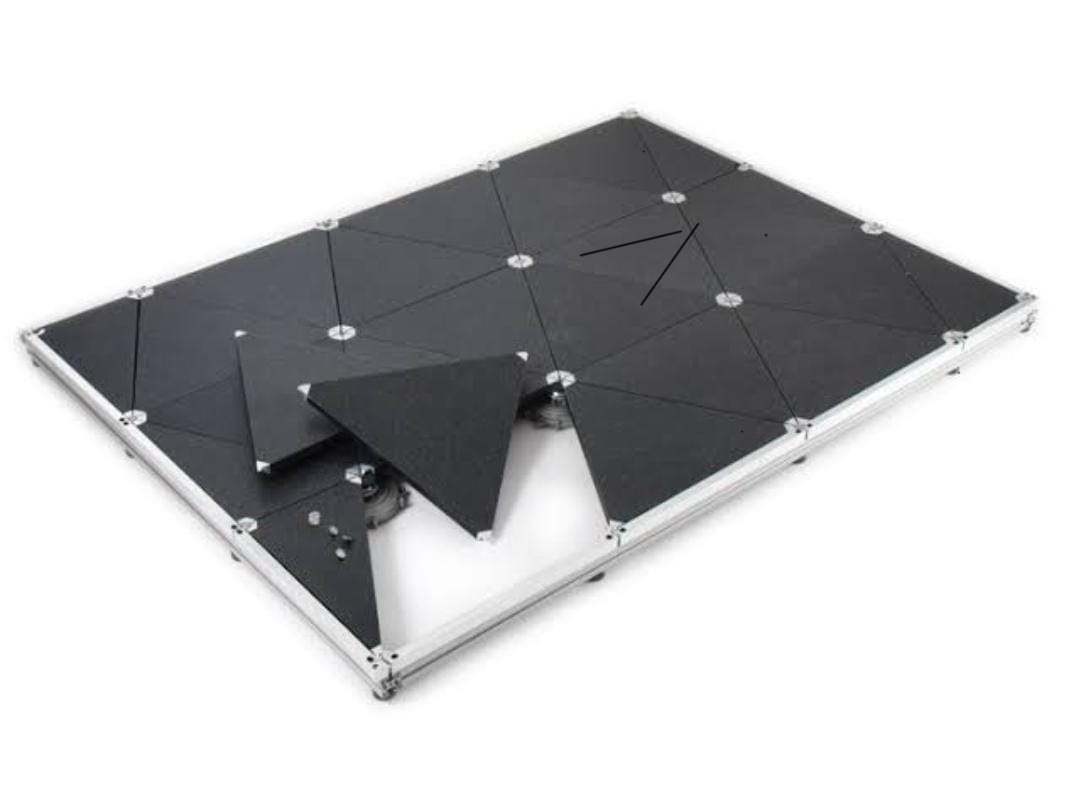
\includegraphics[scale=0.3]{tiles.jpg}
	\caption{Hand Drawn Rough Idea of Working}
\end{figure}
\begin{figure}[H]
	\centering
	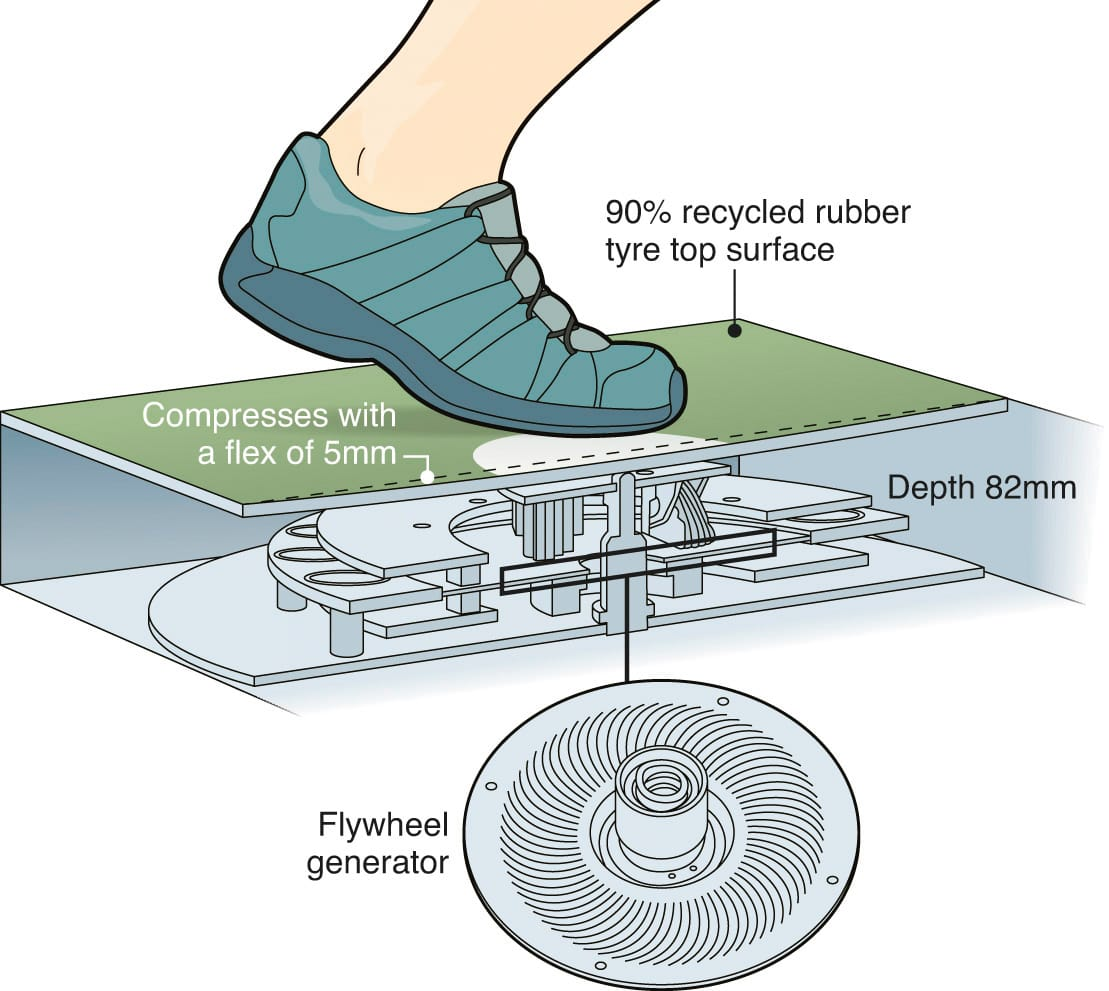
\includegraphics[scale=0.3]{internal.jpg}
	\caption{Hand Drawn Rough Idea of Working}
\end{figure}
\begin{figure}[H]
	\centering
	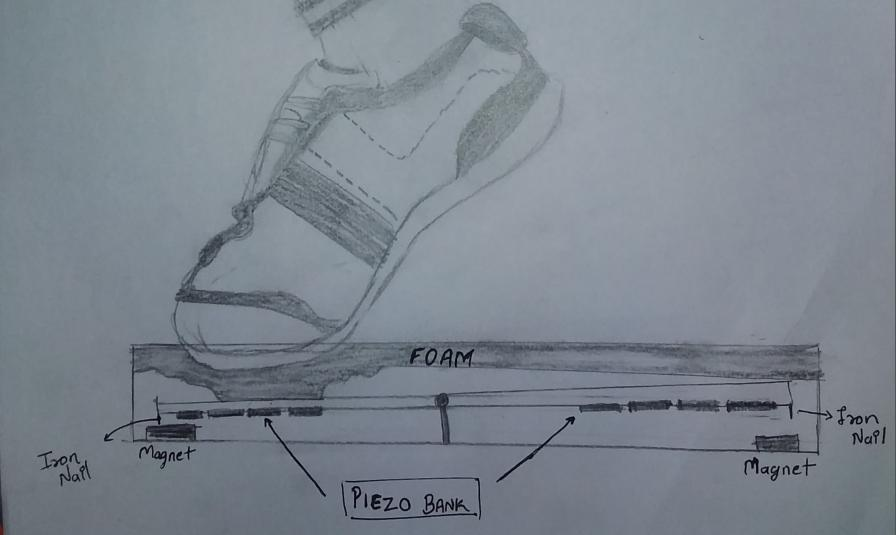
\includegraphics[scale=0.5]{shoe.jpg}
	\caption{Hand Drawn Rough Idea of Working}
\end{figure}
\begin{figure}[H]
	\centering
	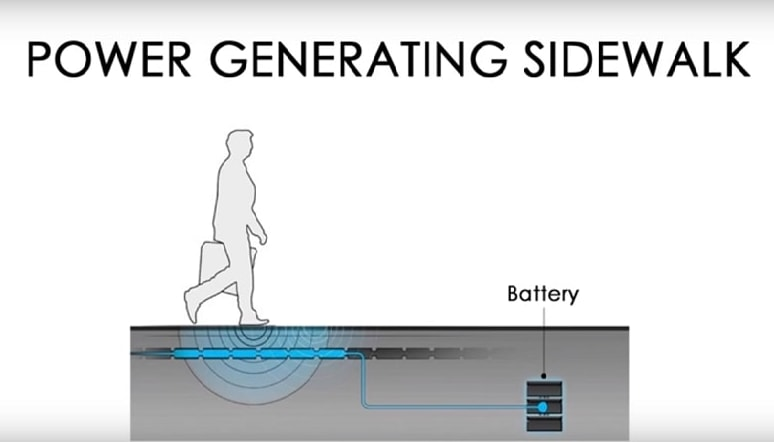
\includegraphics[scale=0.5]{walk.jpg}
	\caption{Hand Drawn Rough Idea of Working}
\end{figure}
\section{Working Explained}
\begin{figure}[H]
	\centering
	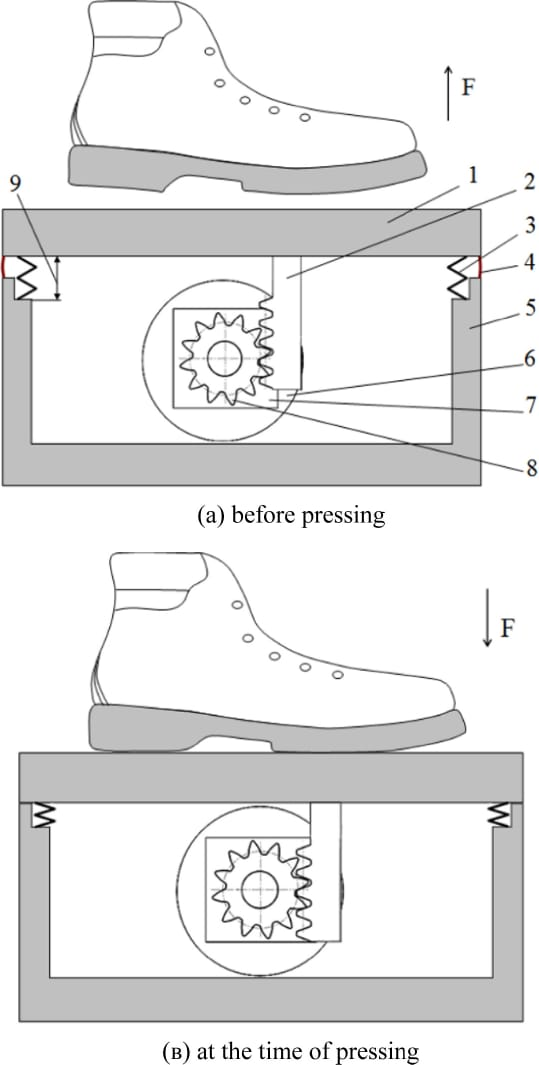
\includegraphics[scale=0.5]{working 1.jpg}
	\caption{Hand Drawn Rough Idea of Working}
\end{figure}
\begin{figure}[H]
	\centering
	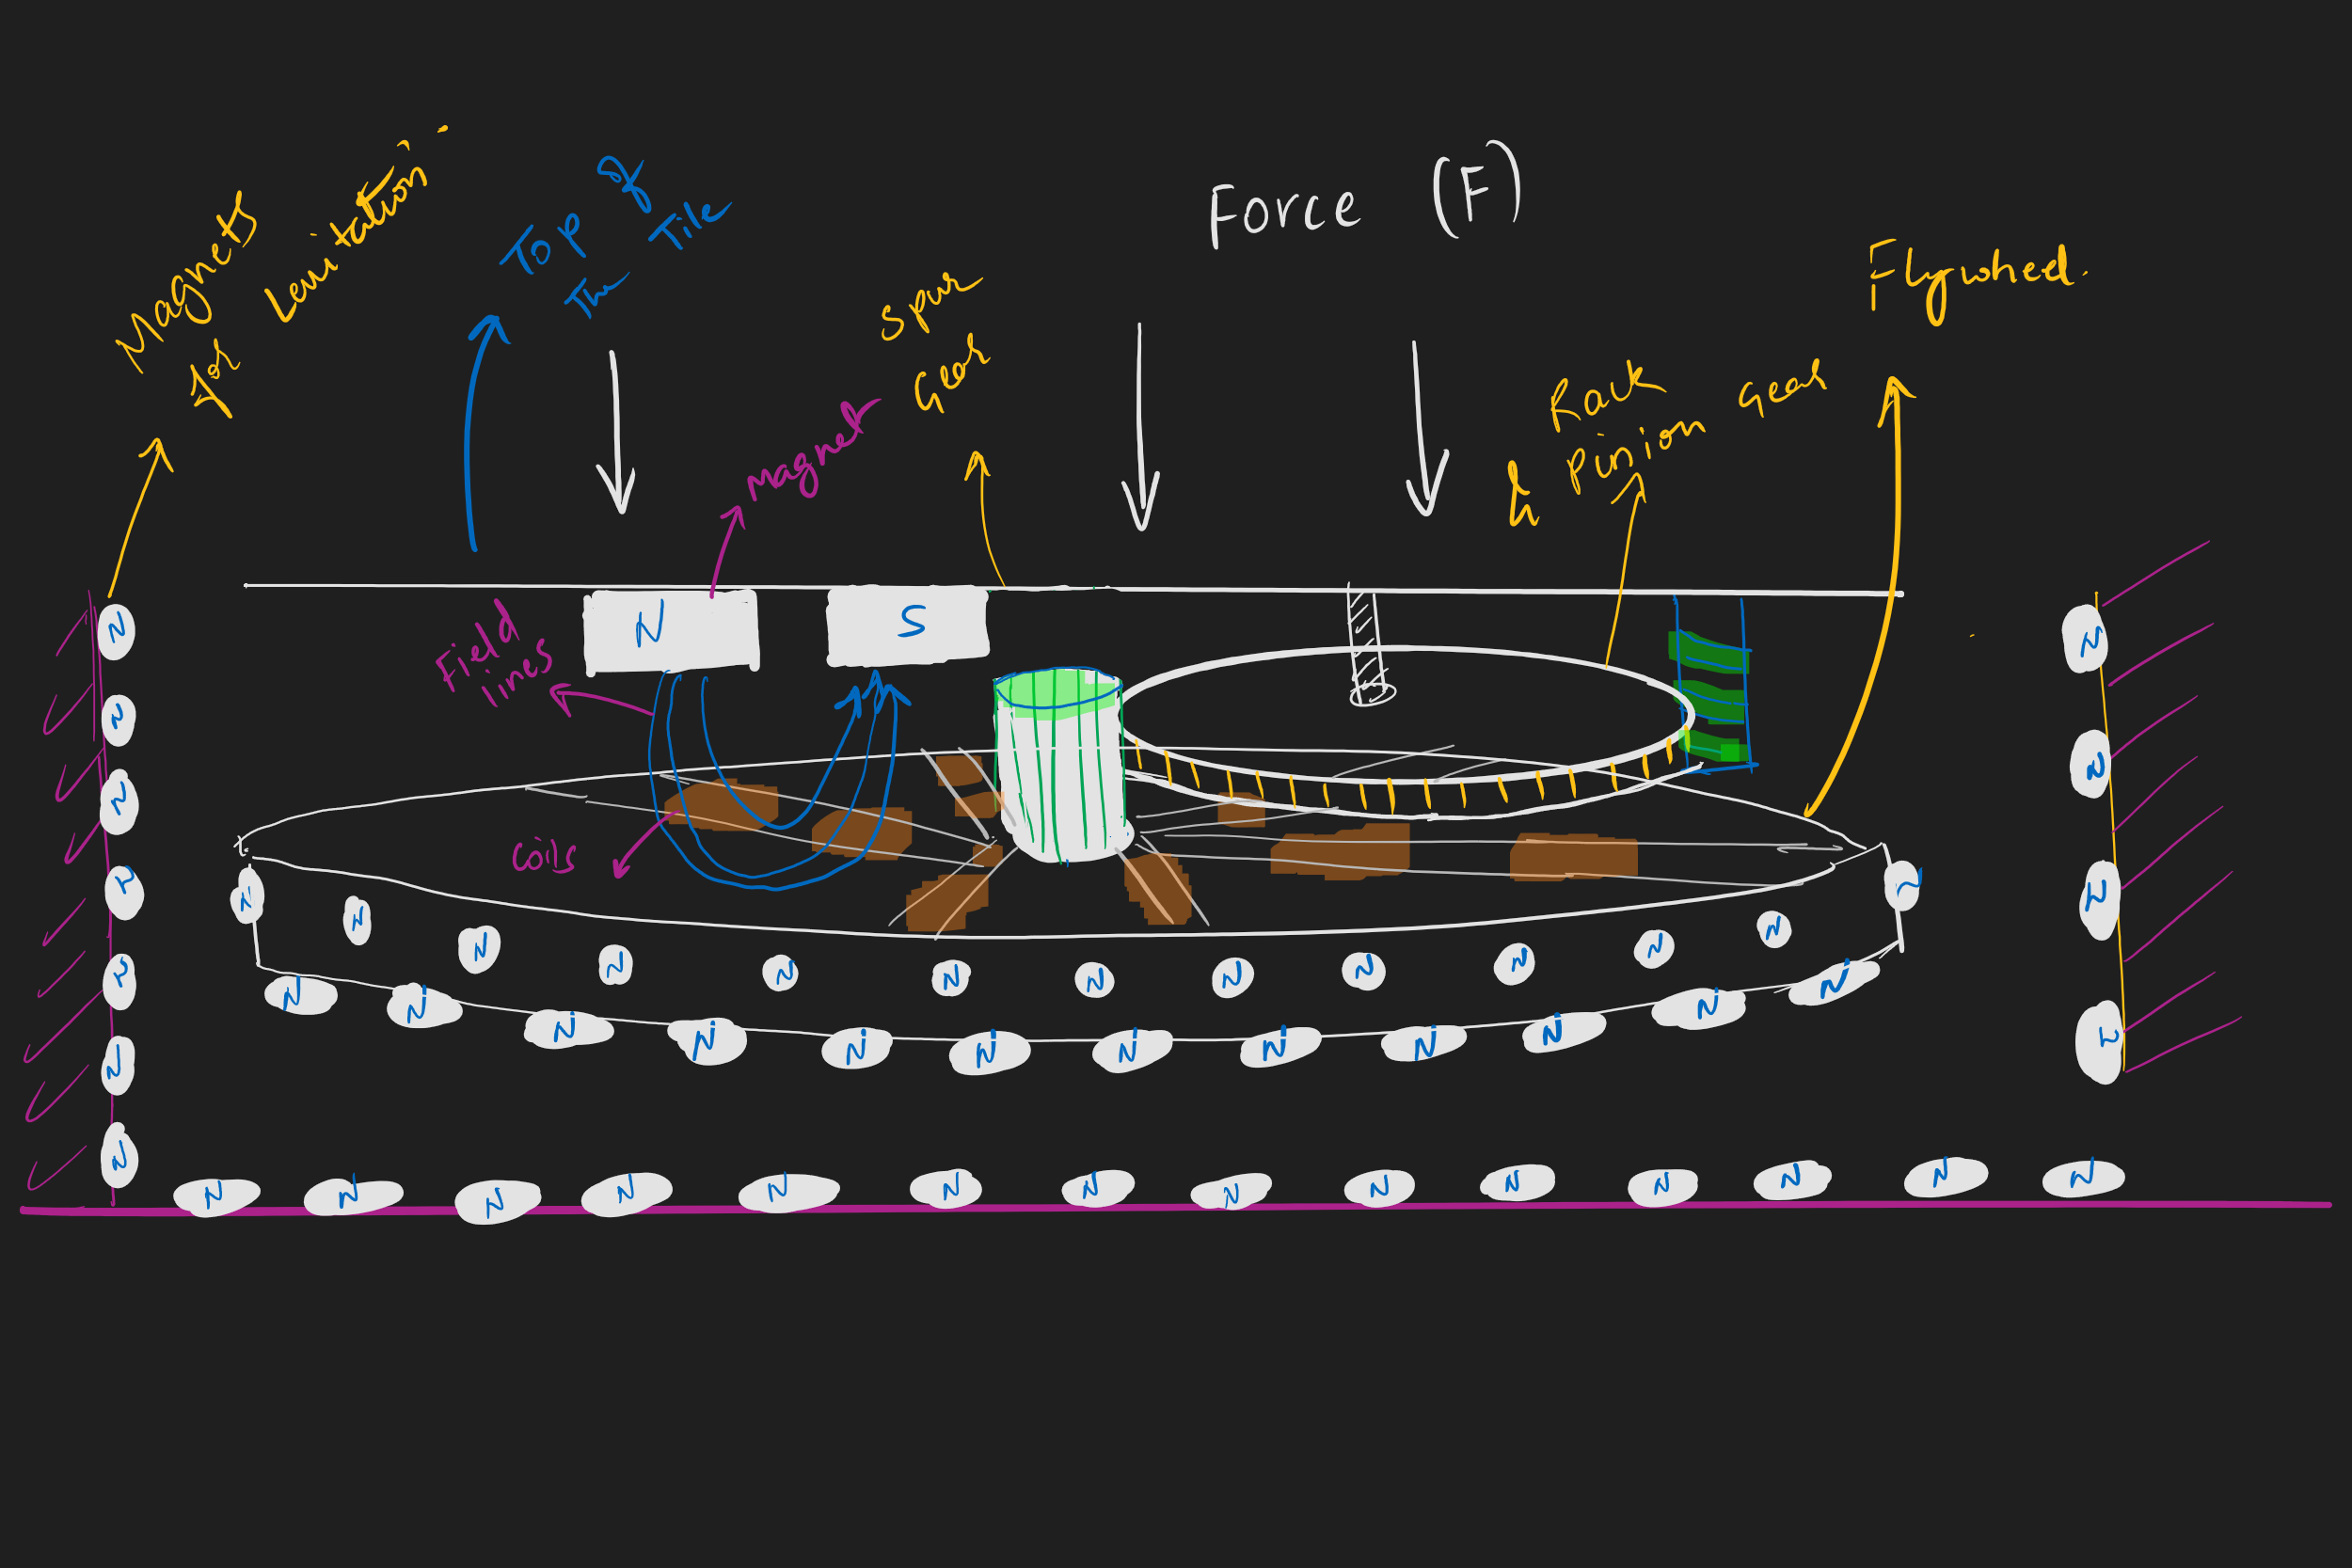
\includegraphics[scale=0.3]{working.png}
	\caption{Hand Drawn Rough Idea of Working}
\end{figure}

As seen in Figure, and in Calculations, The Working is pretty simple. \\

As People Walk on the Roads, paved with these tiles, just 16 Tiles will power a Street Light for one Night. As People Walk, their Potential Energy is used to push against the tile, which rotates a Rack and Pinion Gear that then rotates a Levitating Flywheel, which spins due to the Force and then due to its Inertia.\\

But the Flywheel has lots of coils wrapped around it, and it will therefore produce EMF due to Laws of Electromagnetic Induction when near a Magnet. So We will essentially have a motor that Produces about 20 W of power every day due to just one tile. 

This Power will then be given to the Battery and be stored there by people walking throughout the Day. 


\section{Theoretical Pre-Requisites}
\subsection{Electromagnetic Induction}

\subsubsection{Definition}
Electromagnetic Induction is a current produced because of voltage production
(electromotive force) due to a changing magnetic field. This either happens when a conductor is placed in a moving magnetic field (when using AC power source) or when a conductor is constantly moving in a stationary magnetic field.

\subsubsection{Applications}
Based on his experiments we now have Faraday’s law according to which the amount of
voltage induced in a coil is proportional to the number of turns of the coil and the rate of changing magnetic field.
\begin{enumerate}
	\item AC generator works on the principle of electromagnetic induction.
	\item The working of electrical transformers are based on the electromagnetic
	induction.
	\item The magnetic flow meter is based on the electromagnetic induction.
\end{enumerate}

$$ E = N* \frac{d\phi}{dt} $$

\subsection{Fly Wheels}
\subsubsection{Definition}
Flywheel is a mechanical device which uses the conservation of angular momentum to
store rotational energy; a form of kinetic energy proportional to the product of its
moment of inertia and the square of its rotational speed. Common uses of a flywheel
include: Smoothing the power output of an energy source.

A flywheel is a mechanical device which stores energy in the form of rotational
momentum. Torque can be applied to a flywheel to cause it to spin, increasing its
rotational momentum. This stored momentum can then be used to apply torque to any
rotating object, most commonly machinery or motor vehicles.

In the case of motor
vehicles and other moving objects, the rotational inertia of the flywheel can have an effect due to gyroscopic motion, resisting a change in the direction of the vehicle. If the mass of the flywheel is significant compared to the overall mass of the vehicle, turning and stopping the vehicle is difficult. This fact means careful design of a flywheel is required for application in moving vehicles
\subsubsection{Applications}
Flywheels are often used to maintain consistent energy where the normal energy source
is intermittent. For example, a flywheel can be connected to the crank shaft of a engine
(assuming a manual transmission), storing rotational energy while torque is applied.
When the torque is removed, the flywheel can continue to apply torque to the drive shaft,
giving the engine a more consistent power output

\subsection{Friction}
Friction is defined as the contact resistance exerted by one body upon a second body
when the second body moves or tends to move past the first body.Friction is a retarding
force always acting opposite to the motion or tendency to move.\\

Whenever a tendency exists for one contacting surface to slide along another surface the friction forces
developed are always in a direction to oppose this tendency.a)In some types of machines
we want to minimize the retarding effect of friction forces.\\

Examples : bearings of all
types, power screws, gears, flow of fluid in pipes, propulsion of aircraft, missiles through
the atmosphere.b)In some situations we wish to maximize the effect of friction as in
brakes, clutches, belt drives and wedges. Wheeled vehicles depend on friction for both
starting and stopping and ordinary walking depends on friction between the shoe and
ground.
Friction is used in car brakes, when we walk or climb a hill, making a fire, skiing down a
hill, and more.
\subsection{Force}
\subsubsection{Definition}
Force is a push or a pull that changes or tends to change the state of rest or uniform
motion of an object or changes the direction or shape of an object. It causes objects to
accelerate. Force is an external agent capable of changing the state of rest or motion of a
particular body. It has a magnitude and a direction. The direction towards which the force
is applied is known as the direction of the force and the application of force is the point
where force is applied
\subsubsection{Applications}
In physics, motion is defined as the change in position with respect to time. In simpler
words, motion refers to the movement of a body. Typically, motion can either be
described as:
\begin{enumerate}
	\item Change in Speed
	\item Change in Direction
\end{enumerate}
The Force has different effects and here are some of them.
\begin{enumerate}
	\item Force can make a body that is at rest to move.
	\item It can stop a moving body or slow it down.
	\item It can accelerate the speed of a moving body.
	\item It can also change the direction of a moving body along with its shape and size
\end{enumerate}


\pagebreak
\section{Power Generation Estimates}

\subsection{Calculations}
\noindent
On Every step, the tile is pressed \hfill = 1 cm.\\
Number of Teeth on the Rack and corresponding Pinion Gear\\
That will be travelled in that 1 cm \hfill= 5 (say)\\
Number of Turns on Each Coil\hfill = 500\\
Number of Coils = 5
Magnetic Field\hfill = B = 0.1 T\\
Area \hfill= 20 cm x 10 cm\\
Time taken for one rotation\hfill = 0.2 s\\
Total Rotations \hfill= 5\\
So Electromagnetic Induction \\
$$ E = 5 * N* \frac{d\phi}{dt} $$
E = 100 V for Each Step\\

\noindent
Resistance in the Wires, Battery and Circuit\hfill= 500 $ \Omega $\\
Current \hfill= 100/500 = 0.2 A\\
Power \hfill= 100 * 0.2 = 20 W\\

\noindent
Time Walked by People in a Day \hfill = 10 Mins\\
With each push, the Flywheel, due to inertia will spin for \hfill = 1 Min\\
Number of Estimated Steps \hfill = 500\\
so Time Spun in Total with coils \hfill = 3 Hours in a Day\\

\noindent
Energy in the Battery \hfill = 20W * 3H = 60 Wh\\
Cheap and Efficient LED Tubelights \hfill= 20W\\
Brighter LED Street Lights \hfill = 100W\\
Time Required to Last \hfill = 10 Hr\\
Energy Needed by One Street Light \hfill = 100W * 10 = 1 Kwh = 1 Unit Daily.\\
So Tiles Needed \hfill =  1000/ 60 = \textbf{16 for Each Street Light Per Night.}\\

\section{Materials and Components}
\subsection{Materials}
The tiles are made from nearly 100-percent recycled materials (mostly rubber) and some marine grade stainless steel. 

They can be retrofitted to existing structures and are waterproof as well as designed to withstand outdoor conditions. The tiles are completely waterproof, so they can endure rain, snow, and ice.

Tile are made from recycled polymer, with the top surface made from recycled truck tires.
\pagebreak

\subsection{Components}

\begin{enumerate}
	\item Heavy Metal Flywheel
	\item Magnets
	\item Coils
	\item Battery
	\item Gears
	\item Circuit Board
	\item Controller IC
	\item Protection IC
\end{enumerate}

\subsection{Pricing}
These tiles, from manufacturing to installation costs about 5000 Rs -12000 Rs per square foot. With more localization these tiles would be cheaper and accessible in rural areas.
\section{Potential Advantages}
\begin{enumerate}
	\item Environment Friendly
	\item Controls Climate pollution and global warming
	\item Streets wont be dimly lit, and so will be safer and prevent crimes. 
	\item Cost Efficient
	\item Will make use of the Energy expended by vehicles and people walking.
	\item Recycling materials.
\end{enumerate}

\section{Rooms for Improvement}
\begin{enumerate}
	\item Reduce Resistance in Circuit and Wires to Increase Power
	\item Increase number of coils to increase EMF Generated.
	\item Use more Efficient LED Lights.
\end{enumerate}


\section{Conclusion}
It was a learning Experience, and the Process of Designing a Product and Finding a Solution to a Problem statement was understood. A Product was Designed and the Problem Statement was provided a viable solution to. 
\subsection{Results}
It was found that Each Tile can produce about 20W of power in a day. For one Streetlight we would just need 16 tiles.

\pagebreak
\begin{thebibliography}{}
	
\bibitem{s1}
LED Street Lights\\
\url{https://blogs.worldbank.org/energy/led-street-lighting-unburdening-our-cities}	
\bibitem{s1}
Electromagnetic Induction\\
\url{https://www.niehs.nih.gov/health/topics/agents/emf/index.cfm}	
\bibitem{s1}
Flywheel Battery\\
\url{https://www.youtube.com/watch?v=yhu3s1ut3wM}	
\bibitem{s1}
Pavegen\\
\url{https://pavegen.com/}	
\bibitem{s1}
Inertia and Mass\\
\url{https://www.physicsclassroom.com/class/newtlaws/Lesson-1/Inertia-and-Mass}	
















\end{thebibliography}
	
	
\end{document}